\tikzstyle{rfid}=[draw=none, fill=blue, fill opacity=0.7, text opacity=1, circle, minimum size=0.6cm]
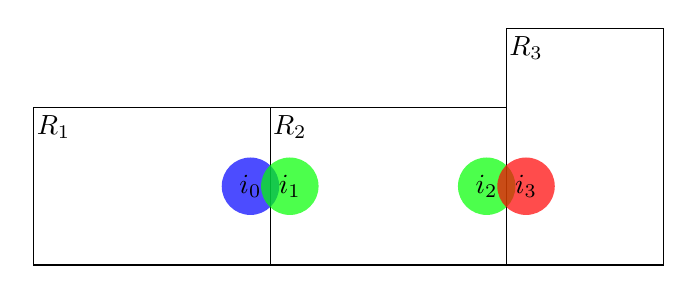
\begin{tikzpicture}[scale=0.5]

\draw  (0,0) rectangle (4,6);
\node at (0.5,5.5) {$R_3$};

\draw  (0,0) rectangle (-6,4);
\node at (-5.5,3.5) {$R_2$};

\draw  (-6,0) rectangle (-12,4);
\node at (-11.5,3.5) {$R_1$};

\node[rfid] at (-6.5,2) {$i_0$};
\node[rfid,fill=green] at (-5.5,2) {$i_1$};

\node[rfid,fill=green] at (-0.5,2) {$i_2$};
\node[rfid,fill=red] at (0.5,2) {$i_3$};

\end{tikzpicture}